\documentclass[12pt]{article}
\usepackage[margin=1in]{geometry}
\usepackage{amssymb}
\usepackage{amsmath}
\usepackage{amsthm}
\usepackage{amsfonts}
\usepackage[shortlabels]{enumitem}
\usepackage{mathtools} 
\usepackage{amscd}        % For simple commutative diagrams
\usepackage{graphicx}
\usepackage{rotating}     % To rotate figures, tables, ...
\usepackage{color}
\usepackage{pdfpages}
\usepackage{blkarray, bigstrut, multirow}
\usepackage{hyperref}


\begin{document}
\begin{titlepage}
    \begin{center}
        \vspace*{1cm}

        \textbf{Winning with Arclight Phoenix}

        \vspace{0.5cm}
        The way of the Bird

        \vspace{1.5cm}

        \textbf{Josh Mulloy}

        \vspace{0.8cm}

        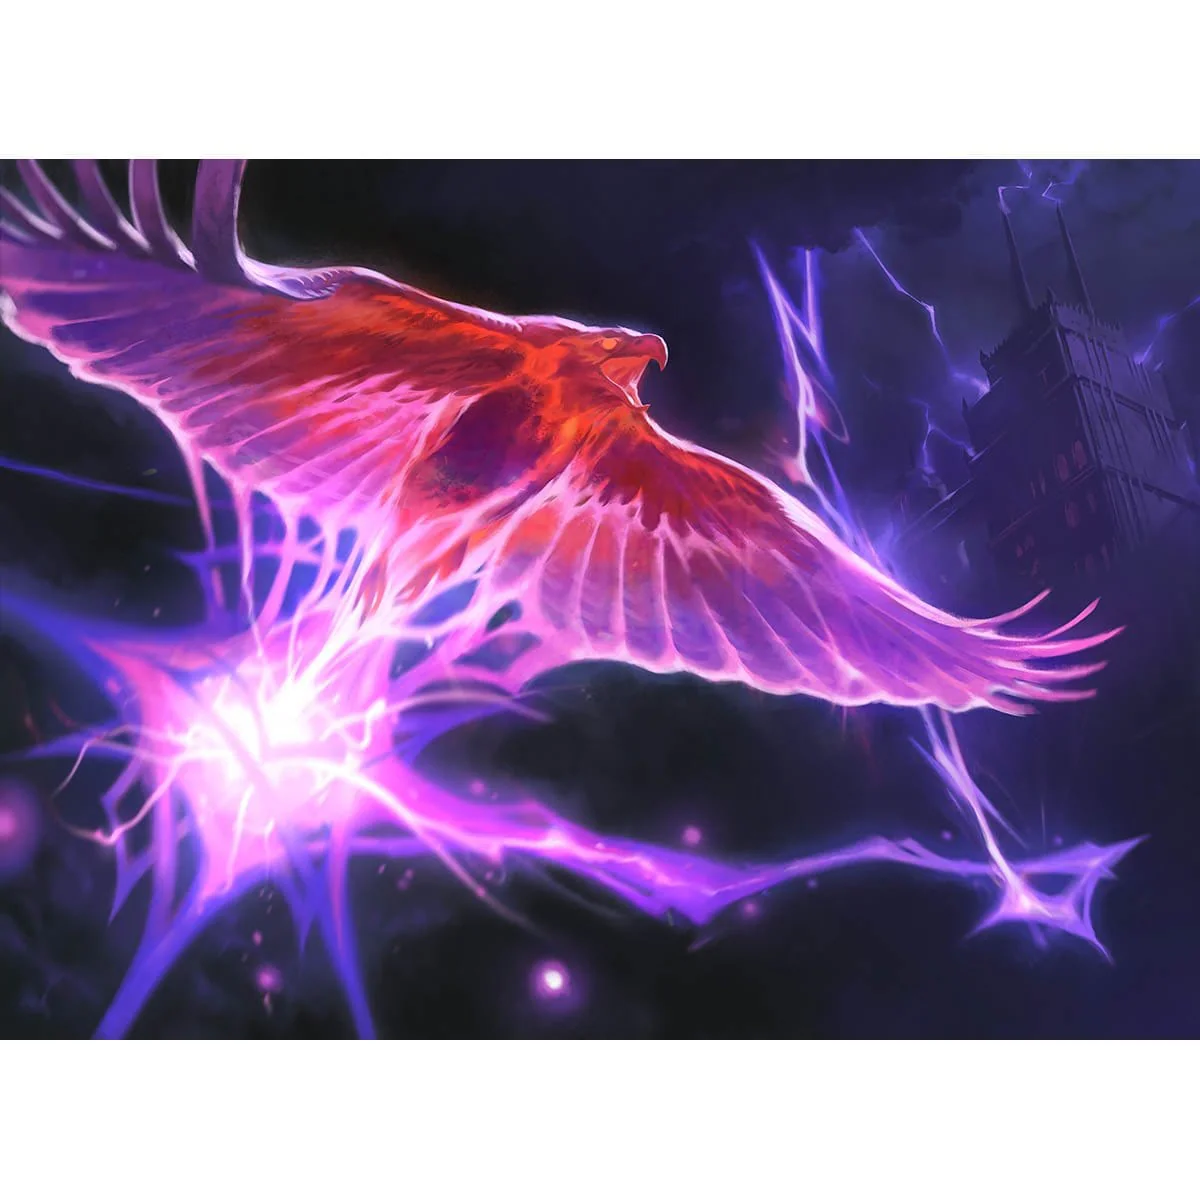
\includegraphics[width=0.7\textwidth]{arclight}

        \vfill

        A guide to playing arclight phoenix\\
        from a mid player
    \end{center}
\end{titlepage}

\tableofcontents

\clearpage
\section{Current List}
\begin{center}
    \href{https://www.mtggoldfish.com/deck/6561022#online}{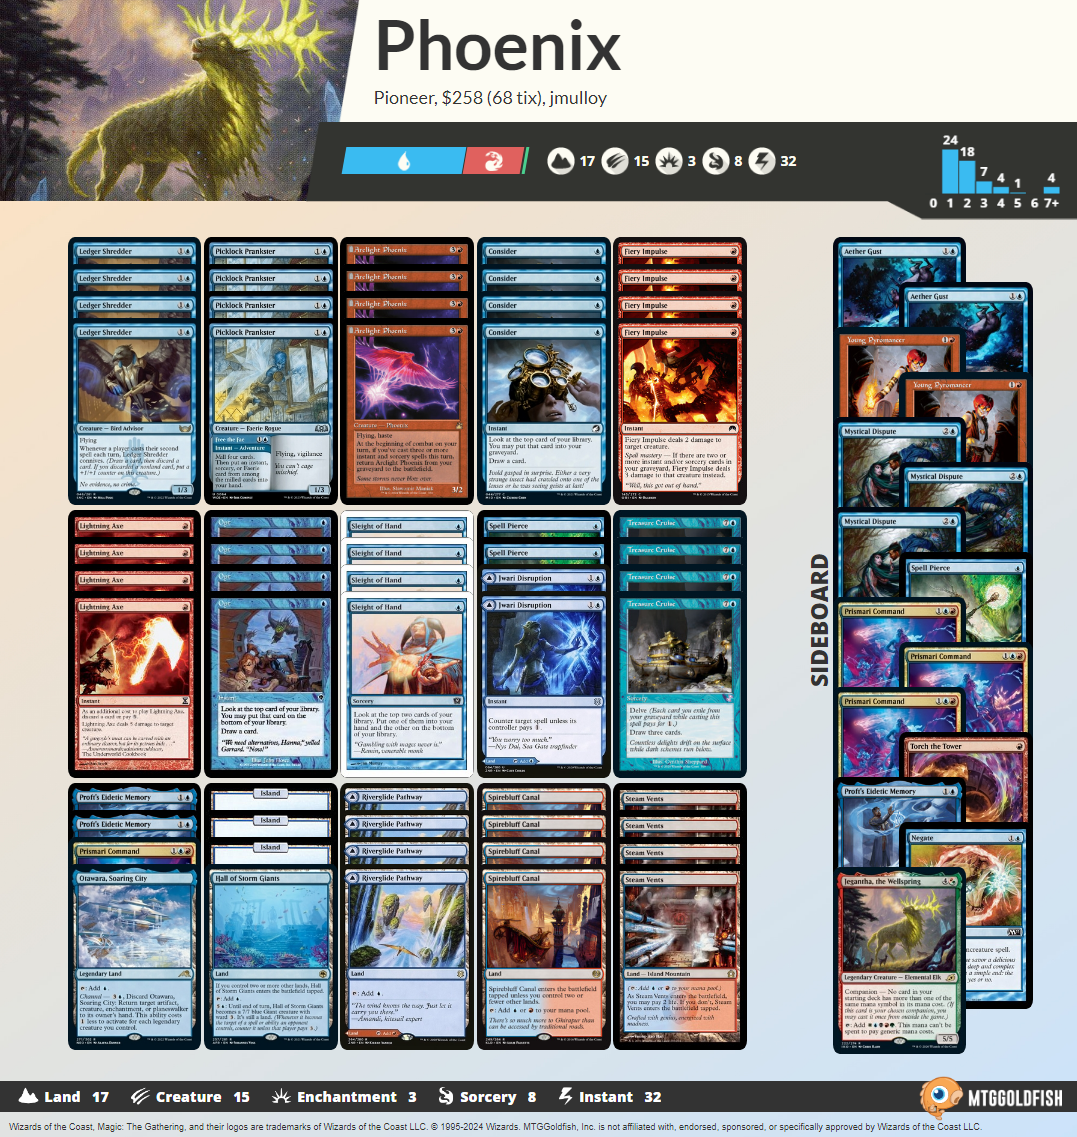
\includegraphics[width=1\textwidth]{decklist}}

    \href{https://www.mtggoldfish.com/deck/6561022}{https://www.mtggoldfish.com/deck/6561022}

    \vspace{0.5cm}

    \href{https://docs.google.com/spreadsheets/d/1DheUoGrQmpuwzbMDpPVJHcCrfe7UOyXSMSSkL8aXnv0/edit?usp=sharing}{Phoenix Matches (started tracking Aug 2024 [Challenge+ level]):}

    \href{https://docs.google.com/spreadsheets/d/1DheUoGrQmpuwzbMDpPVJHcCrfe7UOyXSMSSkL8aXnv0/edit?usp=sharing}{Spreadsheet Link}
\end{center}

\clearpage
\section{Why Phoenix?}
\subsection{Card Velocity}

\subsection{Low vs. High Resource Games}

\subsection{It is Fun}

\clearpage
\section{The Details}
\subsection{Cantrip Sequencing}

\subsection{Playing Ledger Shredder}

\subsection{Thoughtseize}

\subsection{Graveyard Hate}

\subsection{Mulliganing}

\clearpage
\section{Card Choices}
\subsection{Main Deck Cards}
\label{sec:mainchoices}
Jegantha:
Much better than I expected it to be. Really good as just a card that can be put in hand to pitch to axe/shredder. Also fine as a beater in the low resource games.

Proft:
Trespass plays pretty poorly with prankster, while this plays really well. Pretty sure this is just better in the mirror too. Definitely reduces our combo potential, making it a bit more important to chip in for damage when possible compared to the old phoenix lists, but you can still use this to kill people out of nowhere.

Cantrips:
Seen lists playing 3 sleight, 4 opt, 4 consider. Do not do this if you want to win.

Spell Pierce:
Very good against RB with game in the mirror and not dead against amalia. Kinda want to try going down to 2 and playing a md prismari.

Prismari Command:
I feel very close to wanting one of these main, just haven't pulled the trigger yet. See SB section for why I like it.

Lands:
The way I see it, phoenix lists have 4 flex slots for lands, usually choosing between 3rd island, hall of storm giants, jwari disruption, mountain, and stormcarved coast. I like jwari as something to bridge the gap to a turn 3 shredder that also gives us the ability to sometimes steal games by sniping something or making our opponent sequence weird. Hall is similar, where it is just there to shore up some games that we could be losing without it, specifically the low resource ones. I haven't felt a lot of pressure on red sources in my lists so I don't play an additional red source in mountain or stormcarved, but not playing them means you have to be a bit more careful deciding whether to put your pathways on red.

Torch the Tower:
This card isn't better than impulse in basically any mu, including the mirror. I can't see myself ever playing one.

\subsection{Sideboard Cards}
\label{sec:sbchoices}
Prismari Command:
Does everything we want in the low resource games, while also dealing with most of the actually good hate against us. All 4 modes come up often. An important part of casting crusie in low resource post board games to pull ahead, acting as a quadruple lotus petal a lot of the time. Basically, it is a good anti hate card that also just plays really well in the games before, after, and during the hate.

Anger of the Gods:
I never really found myself in spots where I wanted to cast it and often just ended up holding it until it got binned to a shredder. Turning off jegantha wasn't really part of the decision here because jegantha isn't that good against amalia, but it's a nice plus to have it.

Torch the Tower:
See above.


\clearpage
\section{Matchups and Sideboarding}
\subsection{RB Vampires}

\subsection{Phoenix Mirror}

\subsection{Amalia}

\subsection{UW/UB Control}

\subsection{Mono Green}

\subsection{Lotus Combo}

\subsection{Spirits}

\subsection{Niv/Enigmatic}

\subsection{Ensoul}

\subsection{Red Aggro}

\subsection{GB Food}

\subsection{RB Sac}

\end{document}